\documentclass[8pt]{article}
%%%%%%%%%%%%%%%%%%%%%%%%%%%
% Packages
%%%%%%%%%%%%%%%%%%%%%%%%%%%
\usepackage{hyperref}
\hypersetup{
  pdfauthor={Marco Arieli Herrera-Valdez},
  pdftitle={}
  pdftex,
  colorlinks=true,
  urlcolor=Bittersweet,
  linkcolor=blue,
  pdftoolbar=true,
  pdfmenubar=true,
  citecolor=Purple,
  filecolor=blue,
}
%\usepackage[spanish,es-nodecimaldot]{babel}
\usepackage{lscape}
\usepackage{setspace}
%\setstretch{1.1}
%\doublespacing
\usepackage[utf8]{inputenc}
%\usepackage[latin1]{inputenc}
%\usepackage[applemac]{inputenc}
%% Only if the base font of the document is to be different, say sans serif
% Text layout
\usepackage[T1]{fontenc}
\usepackage[scaled=0.92]{helvet}
\renewcommand*\familydefault{\sfdefault}
\usepackage{authblk}
\usepackage{graphicx}
\usepackage{python}
\usepackage{mathtools,amsfonts,amssymb,amsmath}
\usepackage[dvipsnames,svgnames,hyperref,table]{xcolor}
%\usepackage{xcolor}
\usepackage{microtype}
\usepackage{sidecap}
%\hypersetup{pdfpagemode=FullScreen}
%\usepackage[left=2.5cm,right=2.5cm,top=0cm,bottom=2cm,includehead]{geometry}
\usepackage{geometry}
\usepackage{fancyhdr}
%\pagestyle{fancyplain}
%\pagestyle{plain}
% The color packages must appear before the pdfpages package
%\usepackage{chemarr}
\usepackage{listings}
%\usepackage[normalem]{ulem}
%\usepackage[usenames,svgnames,dvipsnames]{xcolor}
%\usepackage[dvipsnames,svgnames,usenames]{xcolor}
%\usepackage{booktabs} % Top and bottom rules for table
\usepackage[font=small,labelfont=bf]{caption}
%\usepackage{wrapfig}
%\usepackage{subfigure}
%\usepackage{beamerthemesplit}
\usepackage{boldline}
\usepackage{multirow}
\usepackage{multicol}
\usepackage{longtable}
\usepackage{times}
\usepackage{animate}
\usepackage{pdfpages}
\usepackage{url}
%\usepackage{multimedia}
%\usepackage{movie15}
%\usepackage{media9}
\usepackage{verbatim}
%\usepackage{pgflibraryarrows}
%\usepackage{pgflibraryshapes}
\usepackage{tikz}
%\usetikzlibrary{arrows,shapes,matrix,chains,calc,positioning}
%\usetikzlibrary{trees,mindmap}
\usepackage{ifthen}
\usepackage{animate}

% To get the envelope in the author list
\usepackage[misc]{ifsym}
%\usepackage[misc,geometry]{ifsym}

%\Letter after the name of the corresponding author

% --------------------------------------
% Bibliography
% --------------------------------------
%\usepackage[sort&compress]{natbib}
\usepackage[round,sort&compress]{natbib}
%\usepackage[numbers,sort&compress]{natbib}
%\bibliographystyle{plainnat}

/Users/curandero/docsLaTeX/mahvLaTeXCommands.tex
\usepackage[utf8]{inputenc}
\usepackage[position=top]{subfig}
\usepackage{tkz-berge}
\usetikzlibrary{arrows,petri,topaths}
\tikzstyle{vertex}=[circle, draw, inner sep=3pt, minimum size=5pt]
\newcommand{\vertex}{\node[vertex]}
\setstretch{1.3}
%
\title{Dinámica inicial de la epidemia de Covid-19 en en mundo y en México }
\author{Marco Arieli Herrera-Valdez}
\date{April 2020}
%
\begin{document}
%
%\begin{flushleft}
%\begin{Large}
%{Estimaciones y análisis de la dinámica inicial de la mortalidad de casos epidemia de Covid-19 en México a partir de los datos mundiales}
%\end{Large}\\
%\smallskip
%\begin{large}
%Carlos Ignacio Herrera-Nolasco$^1$, Eugenia O'Reilly-Regueiro$^{4,\email}$,
%Marco Arieli Herrera-Valdez$^{1,\email}$
%\end{large}\\
%\smallskip
%$^1$ Departamento de Matemáticas, Facultad de Ciencias, Universidad Nacional Autónoma de México\\
%$^4$ Instituto de Matemáticas, Facultad de Ciencias, Universidad Nacional Autónoma de México\\
%$\email$ marcoh@ciencias.unam.mx, eugenia@im.unam.mx
%\end{flushleft}
%
% ---------------------------------------------------------
\section*{Estudio de dinámica global y local de propagación de COVID-19 con apoyo de modelos estocásticos y en datos globales}
\paragraph{Participantes.} Carlos Ignacio Herrera-Nolasco, Sergio Iván López-Ortega, Marco Arieli Herrera-Valdez. Este reporte técnico es parte de lineas de trabajo que están en proceso de edición para su revisión por pares. Se pueden encontrar más detalles y referencias en \url{https://scab-unam.github.io/dam_COVID-19}.

Los datos presentados aquí fueron obtenidos del 
% !TEX root = tsam_Covid19_Mexico.tex
\subsection*{Inferencia de características del curso temporal de Covid-19 a partir de medidas macroscópicas de reportes de casos, recuperaciones y muertes}


\paragraph{Retrasos entre comienzo de síntomas y recuperación o muerte a partir de los primeros reportes de caso en el mundo}


?`Es posible observar en los reportes de casos hechos a nivel mundial indicaciones del tiempo que tarda una persona en morir por complicaciones de COVID-19 a partir comienza a tener síntomas? Es decir, ?`es posible estimar el retraso en entre la muerte y la manifestación de síntomas desde una perspectiva macroscópica de los casos y los decesos por caso en distintos países? ?`Se puede hacer el mismo tipo de inferencia tomando en cuenta retrasos entre recuperaciones y confirmaciones de caso?


%
\begin{figure}[h]
\begin{minipage}{0.5\textwidth}
\includegraphics[width=\textwidth]{../figures_COVID19_dataAnalysis/dam_COVID19_JHU_delays_AllCountries}
\end{minipage}%
\begin{minipage}{0.5\textwidth}
\includegraphics[width=\textwidth]
{../figures_COVID19_dataAnalysis/dam_COVID19_JHU_delays_caseDeaths}
\end{minipage}%
\caption{Retrasos entre reportes de casos (arriba), muertes (en medio), y recuperaciones (abajo). }. \label{fig:reportArrivals}
\end{figure}


La respuesta está en analizar el retraso entre primer reporte de casos y el primer reporte de muertes en distintos países. La mayoría de los países que primero reportaron casos también reportó muertes (sin retraso). Sin embargo, a medida que pasaron las semanas, se fue observando una tendencia que arroja un retraso promedio de 18 días entre primer caso confirmado y primera muerte en varios países (\figref{fig:reportArrivals}). Es posible medir dicha diferencia utilizando distintos métodos, entre los cuales está simplemente medir la distancia horizontal entre las gráficas acumuladas del número de países que han reportado primer caso o muerte, respectivamente (\figref{fig:reportArrivals}, en medio izquierda, y arriba a la derecha). 
De esa forma también es posible medir el retraso entre reportes de casos y primera recuperación, que resulta ser de aproximadamente 12 días  (\figref{fig:reportArrivals} paneles de abajo).

\bigskip
\paragraph{Contribución de grupos de riesgo por edad a la dinámica de fallecimientos por caso.}
La fatalidad en casos confirmados depende de factores que incluyen la calidad de los servicios de salud, y el acceso a dichos servicios, entre otros. 
Sin embargo, es posible observar algunas similitudes macroscópicas en el comportamiento de las defunciones por COVID-19 en lugares que podría pensarse que los fallecimientos presentarían comportamientos muy distintos , como China y Korea del Sur por un lado, o lugares como Italia, por el otro. 
En Korea del Sur y China, el control es muy estricto y la cuantificación de casos ha sido masiva. 
En cambio en Italia, donde la estructura poblacional es distinta, ha habido más fallecimientos por COVID-19, y ha sido rebasado el sistema de salud al grado de tener que negar el uso de respiradores a la gente. 
Sin embargo, en los tres paises el cociente de fatalidad de casos (CFR por sus siglas en inglés) tiene muchas similitudes (\figref{fig:estimates}, izquierda arriba), que se pueden explotar para obtener las contribuciones relativas de los fallecimientos por COVID-19 (\figref{fig:estimates}, izquierda abajo) por cada grupo de edad al total de muertes observadas, y usar esas estimaciones. 

Por su similitud, es posible usar los pesos relativos de las defunciones de los distintos grupos de edad y  hacer distintas predicciones para el caso de México (\figref{fig:estimates}).


\begin{figure}[h]
\centering
\begin{minipage}{0.5\textwidth}
\includegraphics[width=0.9\textwidth]{../figures_COVID19_dataAnalysis/dam_COVID19_JHU_cfr+propDeathCases_ByAge_China+SKorea+Italy_OneFigure.png}
\end{minipage}%
\begin{minipage}{0.5\textwidth}
\includegraphics[width=0.9\textwidth] {../figures_COVID19_dataAnalysis/dam_COVID19_JHU_cfr+propDeathCasesByAgeTS_EstimatesMexico_subReportFactor12.png}
\end{minipage}
\caption{(Izquierda) Contribuciones de distintos grupos de edad a la fatalidad por casos en China, Korea del Sur, e Italia. (Derecha) Estimaciones de fatalidad para México tomando en cuenta grupos de edad, con los datos de China, Korea del Sur, e Italia, calculado hasta el 11 de abril de 2020, y usando un factor de ajuste por subreporte igual a 12. }\label{fig:estimates}
\end{figure}

Las proyecciones obtenidas usando los datos de los distintos países son similares. Hay que tomar en cuenta que estos datos no han sido ajustados con respecto a subreporte. Por ejemplo, ajustando los datos con un factor de 12 por subreporte, la estimación de  muertes de adultos de más de 70 años para México es  de alrededor 4000 para el 19 de abril de 2020. 


Es importante mencionar que estas estimaciones no toman en cuenta la estructura poblacional en México, o la de los países tomados para el análisis, pero esa información está normalizada en el cálculo de los cocientes de fatalidad por caso (\figref{fig:estimates}). 






% --------------------------------------------------------------------------
\subsection*{Monitoreo de datos de casos, recuperaciones y defunciones desde una perspectiva téorica} 
% --------------------------------------------------------------------------



Después de un análisis preliminar sobre retrasos entre reportes y contribuciones a las defunciones de grupos de edad, es notorio que comportamiento de la prevalencia de casos en distintos lugares del mundo es muy parecido, pese a diferencias en sistemas de salud, estructuras poblacionales, métodos de intervención y vigilancia epidemiológica, etcétera. En particular, las trayectorias de las curvas de casos confirmados, recuperados, y defunciones muestran comportamientos similares a los predichos desde una perspectiva cualitativa con modelos simples de tipo SIR. Lo anterior es cierto para varios países que llevan ya varias semanas reportando casos, y constituye una evidencia de que la dinámica macroscópica (a nivel de país) no varía mucho en el mundo, independientemente de las particularidades de cada lugar. 

Nos enfocamos entonces a la tarea de caracterizar primero la dinámica epidémica en términos generales, tomando en cuenta datos globales, para después hacer estimaciones de carácter puntual que permitan entender mejor el caso de México y plantear estrategias de mitigación, además de estimaciones de eventos importantes como máximos locales de prevalencia, inicio de la epidemia, etcétera. Para hacerlo, tomamos datos de distintos lugares del mundo, estudiamos su dinámica desde una perspectiva teórica (en consideración de predicciones cualitativas hechas por modelos), y obtenemos patrones de comportamiento que nos permitan modelar y estimar distintos escenarios. El último punto se basará en modelaje de la dinámica de COVID-19 a nivel de país, y luego para el caso de México, tomando en cuenta regiones en todo el país. 

\paragraph{?`Es la dinámica de propagación de COVID-19 a nivel de país similar a la predicha en modelos?}

A partir de datos globales (\href{}), calculamos el número básico de reproducción, las prevalencias, incidencias de los datos de distintos países, incluyendo México. 

\begin{figure}[h] \label{Planos fase y obtención de parámetros a partir de dinámica de casos observada en algunos países de Europa}
\begin{tabular}{c}
\includegraphics[width=0.9\textwidth]{../figures_COVID19_dataAnalysis/dam_COVID19_JHU_phasePlane_Spain}
\\
\includegraphics[width=0.9\textwidth]{../figures_COVID19_dataAnalysis/dam_COVID19_JHU_phasePlane_Belgium}
\\
\includegraphics[width=0.9\textwidth]{../figures_COVID19_dataAnalysis/dam_COVID19_JHU_phasePlane_Italy}
\\
\includegraphics[width=0.9\textwidth]{../figures_COVID19_dataAnalysis/dam_COVID19_JHU_phasePlane_Germany}
\end{tabular}
\end{figure}


\begin{figure}[h] \label{Planos fase y obtención de parámetros a partir de dinámica de casos observada en algunos países de Asia}
\begin{tabular}{c}
\includegraphics[width=0.9\textwidth]{../figures_COVID19_dataAnalysis/dam_COVID19_JHU_phasePlane_China}
\\
\includegraphics[width=0.9\textwidth]{../figures_COVID19_dataAnalysis/dam_COVID19_JHU_phasePlane_KoreaSouth}
\end{tabular}
\end{figure}


\begin{figure}[h] \label{Planos fase y obtención de parámetros a partir de dinámica de casos observada en algunos países de América}
\begin{tabular}{c}
\includegraphics[width=0.9\textwidth]{../figures_COVID19_dataAnalysis/dam_COVID19_JHU_phasePlane_US}
\\
\includegraphics[width=0.9\textwidth]{../figures_COVID19_dataAnalysis/dam_COVID19_JHU_phasePlane_Mexico}
\end{tabular}
\end{figure}



\paragraph{Modelo estocástico para definición de intervalos y rangos de acción}
Sea 
\begin{eqnarray}
N(t+h) &=& N(t) - X(t)
 \label{eq:N} \\
I(t+h) &=& X(t) - Y(t)
\label{eq:I}\\
W(t+h) &=& W(t) + Y(t) - D(t)
\label{eq:W}
\end{eqnarray}
donde $X(t)$, $Y(t)$, y $D(t)$ son variables aleatorias entera que representan, respectivamente, la incidencia de infección, los nuevos casos removidos del la cadena de infección al cumplir su periodo infeccioso (recuperados), y los nuevos fallecidos. Los miembros del grupo $W$ ya no participan en la cadena de transmisión. El total poblacional $N+I+T$ no es constante. La dinámica de la epidemia está supuesta como un proceso estocástico no homogéneo en el que no necesariamente hay mezcla homogénea entre infectados y no infectados (Herrera-Nolasco, 2020, En preparación). Las simulaciones están basadas en muestreos binomiales o Poisson, dependiendo de la cantidad de ensayos requeridos en cada muestreo.

 La probabilidad de éxito para cada muestreo puede depender de la cantidad de infectados y su posible contribución (por exposición) a la cadena de transmisión (para $X$), o de tiempos de recuperación y posiblemente muerte (para $Y$). El modelo mostrado en las ecuaciones \eqref{eq:N}-\eqref{eq:W} también permite simular dinámicas epidémicas en poblaciones pequeñas, y controlar de forma independiente  factores como la exposición de los susceptibles al contagio y la contribución de los infectados de distintos grupos, lo que permite considerar escenarios de distanciamiento social, aislamiento de casos sospechosos, aislamiento de casos y la posible contribución de grupos de individuos asintomáticos.





% ---------------------------------------------------------
\subsection*{Estimación de fecha de inicio y pico de la epidemia de COVID-19 en México}


 Por el momento, hemos encontrado regímenes de parámetros al rededor de los cuales podemos simular la dinámica macroscópica de la epidemia en México ajustada con los datos de la Secretaría de Salud de México (\figref{fig:inicioPicoNIW}). Por construcción, sólo una proporción de los susceptibles y una proporción de los infectados están en contacto. Con el fin de dar estimaciones conservadoras de inicio, hemos realizado simulaciones en las que la exposición de susceptibles al contagio es constante, ajustando los datos de la Secretaría de salud  con un factor de 12, y  suponiendo una  población expuesta al 10\%. En esas condiciones, una estimación \textit{conservadora} de la fecha de inicio de la epidemia es aproximadamente 40 días antes del 27 de febrero. Es decir, aproximadamente el 20 de enero de 2020. El pico de la infección estaría estimado para ocurrir al rededor de 75 días después del día 0. Es decir, al rededor de Mayo 14 de 2020. La tendencia de los datos de los últimos días es de crecimiento menor en comparación a las simulaciones. Esto indica que posiblemente haya un retraso aún mayor para observar el pico de la epidemia y con un número de casos menor.
 
 
\begin{figure}[h]
\includegraphics[width=\textwidth]{../figures_COVID19_models/dam_COVID19_Mexico_InitialFit_Herrera-Valdez+Herrera-Nolasco_2020}
\caption{Estimación de la fecha de inicio y pico de la epidemia ajustando los datos iniciales de la epidemia de Covid-19 en México. La fecha cero representa el 27 de febrero de 2020. Para estas simulaciones los infectados de los grupos severo y crítico en las simulaciones tienen exposición nula a otros grupos poblacionales. } \label{fig:inicioPicoNIW}
\end{figure}


 

En esta dirección, ha resultado útil un caso particular del modelo en las ecuaciones \eqref{eq:N}-\eqref{eq:W}  para explorar escenarios en grandes números.
 Para ello, tomamos los valores esperados de los muestreos del modelo estocástico y derivamos una ecuación determinista para el régimen en el que los tamaños poblacionales son grandes (\figref{fig:inicioPicoNIW}). Como resultado obtenemos un modelo que tiene similitud con un SIR clásico.

\bigskip
\begin{minipage}{0.6\textwidth}
De forma explícita, si el tamaño de la población $T=N+I+W$ considerada en el sistema \eqref{eq:N}-\eqref{eq:W} es lo suficientemente grande, es posible derivar un sistema de ecuaciones diferenciales ordinarias para las densidades poblacionales de no-infectados, infectados y removidos, representadas por $x$, $\vec{y}$, y $w$, de tal forma que
\begin{eqnarray*}
\partial_{t} x &=& -  \lambda x\\
\partial_{t} y &=& \lambda x - \vec{\gamma} \cdot \vec{y}  - \delta_{F} y_{C}
\\
\partial_{t} w &=&\vec{\gamma} \cdot \vec{y} + \delta_{F} y_{C}
\end{eqnarray*}
donde $\vec{y}$ y  $\vec{\gamma}$  son  vectores que representan, respectivamente,  los tamaños de la subpoblaciones infecciosas y las tasas de remoción para cada grupo infeccioso. La variable $y$ representa la prevalencia (diaria) de infecciones en la población en el tiempo $t$.
\end{minipage}%
\begin{minipage}{0.4\textwidth}
\centering
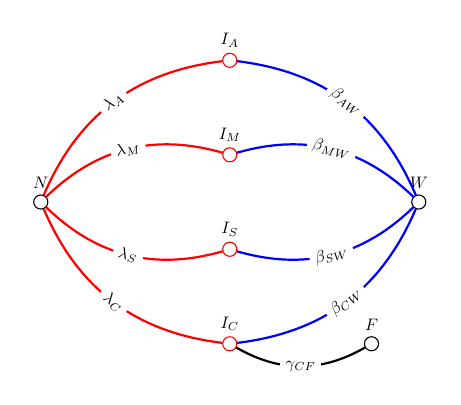
\begin{tikzpicture}[scale=0.6,transform shape]
	\vertex[label=\textcolor{black}{$N$},color=black](N) at (-4,0) { };
	\vertex[label=\textcolor{black}{$I_{A}$},color=red](A) at (0,3) {};
	\vertex[label=\textcolor{black}{$I_{M}$},color=red](M) at (0,1) {};
	\vertex[label=\textcolor{black}{$I_{S}$},color=red](S) at (0,-1) {};
	\vertex[label=\textcolor{black}{$I_{C}$},color=red](C) at (0,-3) {};
	\vertex[label=\textcolor{black}{$W$},color=black](W) at (4,0) { };
	\vertex[label=\textcolor{black}{$F$}](F) at (3,-3) {};
  \tikzstyle{LabelStyle}=[fill=white,sloped]
  \tikzstyle{EdgeStyle}=[bend left]
  \Edge[label=$\lambda_{A}$,color=red](N)(A)
  \Edge[label=$\lambda_{M}$,color=red](N)(M)
  \Edge[label=$\beta_{AW}$,color=blue](A)(W)
  \Edge[label=$\beta_{MW}$,color=blue](M)(W)
  \tikzstyle{EdgeStyle}=[bend right]
  \Edge[label=$\lambda_{S}$,color=red](N)(S)
  \Edge[label=$\lambda_{C}$,color=red](N)(C)
  \Edge[label=$\beta_{SW}$,color=blue](S)(W)
  \Edge[label=$\beta_{CW}$,color=blue](C)(W)
  \Edge[label=$\gamma_{CF}$](C)(F)
\end{tikzpicture}
\end{minipage}%


%\paragraph{Acknowledgments:}


\bibliographystyle{plainnat}
\bibliography{Covid19,epidemiology}
\end{document}
